\documentclass{article}
\usepackage[margin=1in]{geometry}
\usepackage{amsmath, amssymb, amsthm}
\usepackage{enumitem}

% colored links
\usepackage{hyperref}
\hypersetup{
    colorlinks=true,
    linkcolor=blue,
    filecolor=magenta,      
    urlcolor=black!20!BurntOrange,
    }

% strikethrough
\usepackage{soul}

% Inputting Python code
\usepackage[dvipsnames]{xcolor}
\definecolor{textblue}{rgb}{.2,.2,.7}
\definecolor{textred}{rgb}{0.54,0,0}
\definecolor{textgreen}{rgb}{0,0.43,0}
\usepackage{upquote}
\usepackage{listings}
\lstset{
    language=Python, 
    tabsize=4,
    basicstyle={\ttfamily},
    keywordstyle=\color{textblue},
    commentstyle=\color{textgreen},
    stringstyle=\color{textred},
    frame=none,
    columns=fullflexible,
    keepspaces=true,
    showstringspaces=false,
    xleftmargin=-15mm, % manual adjustment, figure out permanent solution
}

% Drawing figures
\usepackage{tikz}
\usetikzlibrary{calc, shapes.symbols}

% Colored Boxes
\usepackage{tcolorbox}
\tcbuselibrary{skins,hooks}
\usetikzlibrary{shadows}
\usepackage{lipsum}

% Quotes
\usepackage{epigraph}

%Images
\usepackage{graphicx}
    \usepackage{subcaption}
    \usepackage{float}

%Formatting and Spacing
\setitemize[1]{noitemsep, parsep = 5pt, topsep = 5pt}
\setenumerate[1]{label = (\alph*), parsep = 1pt, topsep = 5pt}
\setlength\parindent{0pt}
\linespread{1.1}

% title
\title{\vspace{-1cm}CS 2051: Honors Discrete Mathematics \\Spring 2023 Homework 9 Supplement}
\author{Sarthak Mohanty}
\date{}

\begin{document}

\maketitle

\vspace{-1cm}
\section*{Overview}
    One day when I was a student taking CS 2051, I was perusing an \href{https://web.stanford.edu/class/archive/cs/cs103/cs103.1234/timeline_of_results}{article} with all the important results in discrete math. However, I noticed an interesting statement: 
    \begin{tcolorbox}[colframe=gray!40, sharp corners]
        Noam Chomsky invents context-free grammars in his book \textit{``Syntactic Structures"}. At the time, he called them \textit{phrase-structure grammars} and explored them in the context of modeling the syntax of natural languages.
    \end{tcolorbox}
    Initially, I was rather confused. Noam Chomsky may be many things, including a world-renowned linguist and psychologist, but it was difficult to see his correlation to discrete mathematics. However, as I looked more into the topic, I realized the true importance of his discoveries. Chomsky's work has not only transformed the field of linguistics but has also had a significant impact on the entire domain of computer science.

    \vspace{2mm}
    In this supplement, you'll quickly get up to speed (if you aren't already) with a powerful tool known as recursion. You'll use this tool to develop an important computational model, known as a context-free grammar. Finally, using this model, you'll try your hand at algorithmically expressing the English language. Let's get started!

\section*{(Optional) Part 1: Way Down We Go}
\setlength{\epigraphwidth}{0.6\textwidth}
\epigraph{The control of a large force is the same principle as the control of a few men: it is merely a question of dividing up their numbers.}{Sun Tzu, \textit{The Art of War}}
Let's motivate this section by recalling some explication from a prior supplement:

    \begin{center}
        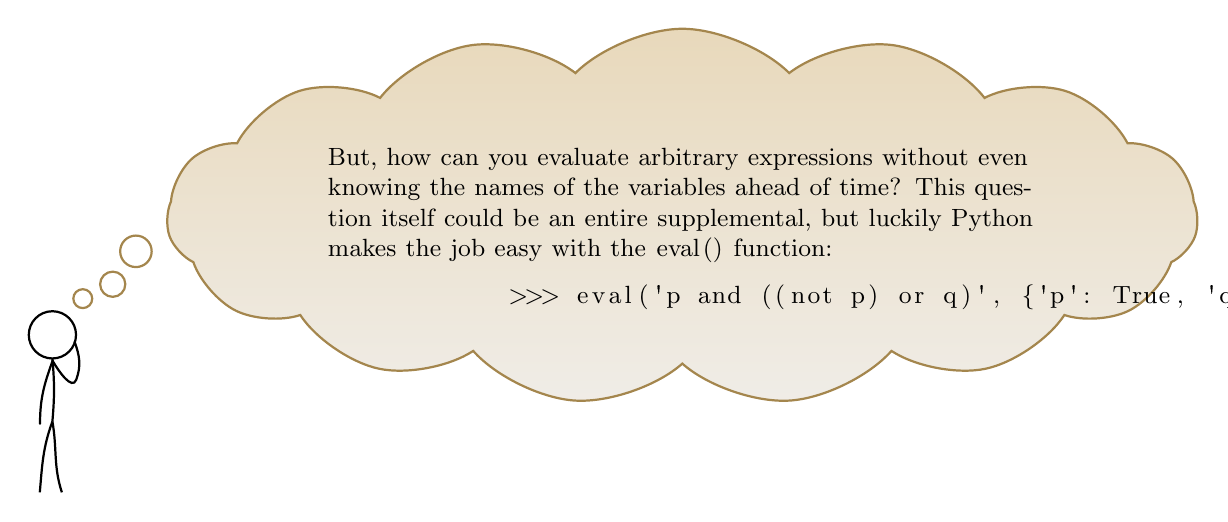
\begin{tikzpicture}
          \def\H{2.0}     % human height
          
          \draw[thick,fill=white] circle (0.15*\H) coordinate (H);
          \draw[thick] (H)++(-90:0.15*\H) coordinate (N) to[out=-85,in=85]++ (0,-0.40*\H) coordinate (P);
          \draw[thick,line cap=round] (N)++(-85:0.03) to[out=-110,in=90]++ (-0.08*\H,-0.4*\H);
          \draw[thick,line cap=round] (N)++(-85:0.03) to[out=-60,in=-110]++ (0.15*\H,-0.12*\H)  to[out=70,in=-70]++ (-0.01*\H,0.24*\H);
          \draw[thick] (P) to[out=-110,in=85] ($(H)+(-0.08*\H,-\H)$);
          \draw[thick] (P) to[out=-80,in=108] ($(H)+(0.06*\H,-\H)$);

          \draw[black!40!Dandelion,thick,fill=white] (H)++(50:0.6) circle (0.06*\H);
          \draw[black!40!Dandelion,thick,fill=white] (H)++(40:1) circle (0.08*\H);
          \draw[black!40!Dandelion,thick,fill=white] (H)++(45:1.5) circle (0.1*\H);

          \node[cloud, thick, draw = black!40!Dandelion, top color=Dandelion!70!black!30,bottom color=Dandelion!40!black!10, aspect=3.5, cloud puffs = 15, cloud puff arc = 90, text width=9cm] (c) at (8,1.5) {\small But, how can you evaluate arbitrary expressions without even knowing the names of the variables ahead of time? This question itself could be an entire supplemental, but luckily Python makes the job easy with the \lstinline+eval()+ function:
        \begin{lstlisting}[belowskip=-10pt]
            >>> eval('p and ((not p) or q)', {'p': True, 'q': False})
        \end{lstlisting}};
    \end{tikzpicture}
    \end{center}
    We now have the opportunity to answer the question we originally posited. How would we go about implementing our own \lstinline+eval()+ function? This problem is not a trivial one, and requires careful consideration of various algorithmic techniques. 
    
    \vspace{2mm}Initially, one may assume that an iterative approach would suffice to traverse the string representation of the proposition, evaluating sub-expressions and gradually building up to the final evaluation. However, such an approach would quickly lead to convoluted code that would be difficult to maintain and debug. Therefore, we turn to a more elegant solution.

    \vspace{2mm}
    \textbf{Recursion} is a powerful tool used for solving algorithms, and is loosely given as follows:
    \begin{itemize}
        \item If the problem is small enough to solve directly, then do so.
        \item Otherwise, reduce it to one or more simpler instances of the same problem.
    \end{itemize}
    There are many advantages to this approach, the main one lying in the fact that the same code can be used to solve both the original problem and its sub-problems, leading to simpler, more modular code.

    \vspace{2mm}
    To apply recursion to the task of creating our \lstinline+eval()+ function, we can break the problem down into two parts. First, we must parse the string representation of the proposition into a data structure that can be easily evaluated, such as a tree. Second, we must recursively evaluate this data structure to arrive at the final evaluation of the proposition.

    % \textbf{Note that there are two different types of recursion involved in this process}. The first type of recursion involves parsing the string representation of the proposition and constructing the tree data structure, while the second type of recursion involves recursively evaluating the subtrees of the tree data structure.
    
    % \vspace{2mm}
    % These two types of recursion correspond to two different types of data structures: \textit{lists} (in the form of strings) and \textit{trees} (in the form of our constructed data structure). This will be explored in future coursework such as CS 351X.

\begin{tcolorbox}[enhanced,interior style={top color=Dandelion!20,bottom color=Dandelion!30}]
    \textbf{Let's build our own \lstinline{eval()} function. Implement the following functions:}
    \begin{itemize}
        \item \lstinline{parse(proposition)}: The function takes in a string, represented as a propositional formula, and parses it to create an appropriate \lstinline{Formula} object. You may assume that the input string is valid.
        \item \lstinline{evaluate(proposition, model)}: This function takes in a string as well as an assignment of variables and returns the evaluation. The output should be identical to that of the analogous built-in function:
        \begin{lstlisting}[belowskip=-10pt]
            >>> evaluate('p and ((not p) or q)', {'p': True, 'q': False})
            False
        \end{lstlisting}
    \end{itemize}

    Note: All functions must be implemented recursively, or call other recursive functions.
\end{tcolorbox}

\section*{Part 2: Models of Computation (10 points)}
    In this section, we introduce an abstract representation for computational machines. \textit{Models of computation} are abstract representations of how computation can be performed. They are commonly used to understand the limits and capabilities of computers and other computational devices. A computational model takes in a string as input, and returns a boolean value that represents whether or not to \textit{accept} that string.

    \vspace{3mm}
    There are several models of computation, such as Turing machines, lambda calculus, and finite automata. In this section we present one such model, known as a \textit{context-free-grammar}. We first introduce the concept through an example, and then formalize the definition.
    
\subsection*{Example 1: Binary strings}
    Let's say we were trying to create a computational model to \textit{decide} the language $L = \{1^{n}0^{n}, n \in \mathbb{N}\}$. What this means is that our computational model should take in a string, and \textit{accept} the string (i.e.\ return \texttt{True}) if the string is in $L$, and \textit{reject} otherwise.

    \vspace{2mm}
    One such model could be represented as follows: we would start with a temporary variable, call it $S$. Now at every time step, keep splitting up $S$ into $1S0$; we can denote this as
    \begin{align*}
        S &\rightarrow 1S0.
    \end{align*}
    Finally, we want to get rid of $S$. Therefore, at every time step, allow the possibility of $S$ to dissapear and be replaced with the empty string, $\epsilon$. We indicate this as follows:
    $$
    \begin{aligned}
        S &\rightarrow 1S0 \\
        S &\rightarrow \epsilon
    \end{aligned}
    \qquad \overset{\mathrm{def}}{=\joinrel=} \qquad S \rightarrow 1S0 \mid \epsilon
    $$
    If we ever generate a string identical to the input we take in, we \textit{accept}, otherwise, we \textit{reject}. Let's informally illustrate why this model decides $L$. Suppose we took in the input string $w = 111000$. Since $w \in L$, our model should accept the string, so our CFG should be able to generate it. To do this, all we have to do is tell our machine to execute the following set of steps:
    $$S \rightarrow 1S0 \rightarrow 11S00 \rightarrow 111S000 \rightarrow 111000.$$ At every time step, we increase the number of $1$s and $0$s on either side of $S$. Finally, when we have generated the desired string, we tell $S$ to disappear, by replacing it with the empty string $\epsilon$.

\subsection*{Context-Free Grammars}
    We now formalize the above concept. A \textbf{context-free grammar} is a 4-tuple $(V, \Sigma, R, S)$. We now explain each of these elements in detail.
    \begin{enumerate}[label = \arabic*.]
        \item $V$ is a finite set called the \textbf{variables}. The elements in $V$ are commonly represented using a capital letter (i.e.\ $A, B, \dots$). In the above example, the only variable was $S$.
        \item $\Sigma$ is a finite set, disjoint from $V$, called the \textbf{terminals}. These can be any symbol; in Example 1, they were the binary numbers $0, 1$.
        \item $R$ is a finite set of \textbf{rules}. The left hand side of a rule is a single variable, and the right hand side can be any combination of variables and terminals.
        \item $S \in V$ is the start variable.
    \end{enumerate}
    The language of the grammar is then $L_{\textsf{CFG}} = \{w \in \Sigma^{*} : S \rightarrow u_{1} \rightarrow u_{2} \rightarrow \dots \rightarrow w\}$\footnote{Here the \href{https://en.wikipedia.org/wiki/Kleene_star}{kleene star} was used to define $w$ as the concatenation of terminals.}. Put another way, it is the set of all valid strings generated by repeated application of our rules containing no variables.

\subsection*{Example 2: Union of Two Languages}
    Let's say we were trying to create a CFG for the language $$L = \underbrace{\{0^{n}1^{n} \mid n \ge 0\}}_{L_{1}} \cup \underbrace{\{1^{n}0^{n} \mid n \ge 0\}}_{L_{2}}.$$ First, let's construct a grammar for $L_{1}$. This is the same as in Example 1: $$S_{1} \rightarrow 0S_{1}1 \mid \epsilon.$$ Similarly, we can generate a grammar for $L_{2}$: $$S_{2} \rightarrow 1S_{2}0 \mid \epsilon.$$ Then we can generate our desired language $L$ with a CFG by `combining' the two grammars, as follows:
    \begin{align*}
        S &\rightarrow S_{1} \mid S_{2} \\
        S_{1} &\rightarrow 0S_{1}1 \mid \epsilon \\
        S_{2} &\rightarrow 1S_{2}0 \mid \epsilon
    \end{align*}

\subsection*{Example 3: RNA Secondary Structure}
        % \footnote{adapted from \href{https://courses.cs.washington.edu/courses/cse311/19sp/hws/homework07.pdf}{here}}
        CFGs were applied successfully to RNA secondary structure prediction in the early 90s. We can get a taste of this application through the following scenario. 
        
        \vspace{3mm}Each RNA string is a string over the alphabet $\{A, C, G, U\}$. The string GUGCCACGAUUCAACGUGGCAC can fold into a lollipop shape like so:
        \begin{center}
            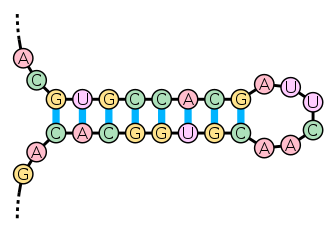
\includegraphics[scale = 0.4]{images/stem-loop.png}
        \end{center}
        The prefix GUGCCACG and suffix CGUGGCAC can together form the handle of the lollipop because they line up in such a manner that As are across from $U$s (or vice versa) and Cs are across from $G$s (or vice versa). The candy part of the lollipop consists of the string AUUCAA, which has length 6.

        \vspace{3mm}In general, an RNA string can fold into a lollipop shape if it can be written as $xyz$, where $x$ and $z$ contain at least two characters each, $y$ contains at least four characters, and the characters of $x$ match up with those of $z^{R}$ (the reverse of $z$), in the sense that that corresponding pairs of letters fall in the set $\{(A, U), (U, A), (C, G), (G, C)\}$. Can you find a CFG to successfully accept such strings?

\subsection*{Induction vs Recursion}
    As a side note, you might be wondering why we introduced recursion in this supplement, when the current focus of the course this week is induction. This is because the two are actually deeply intertwined. \textbf{Induction is often used to prove the validity of recursive models}.

    \vspace{2mm}
    For example, let's try to prove Example 1 using induction. We wish to prove that $$L = L(G),$$ where $L(G)$ is the language of $G$. We do so in two parts.

    \vspace{2mm}
    \textsc{Part 1.} We first prove $L \subseteq L(G)$; in other words we prove $P(n)$, the statement $$\text{Every string of the form $1^n0^n$ can be generated by the CFG.}$$
    \begin{enumerate} [label = {}, leftmargin = .25in]
        \item \textsc{Base Case:} $P(0)$ is true, since we can apply the rule $S \rightarrow \epsilon$ to generate the string $1^{0}0^{0} = \epsilon$.
        \item \textsc{Inductive Step:} Let $n \in \mathbb{N}$ such that $P(n)$ is true. To generate a string of the form $1^{n+1}0^{n+1}$, apply the first production rule $S \rightarrow 1S0$ once, obtaining the string $1S0$. Now we can replace $S$ with $1^{k}0^{k}$, which we know can be generated by the CFG by the inductive hypothesis. Thus, we obtain the string $1^{k+1}0^{k+1} \in L$, so $P(k + 1)$ is true.
        \item \textsc{Conclusion:} Therefore by induction, $P(n)$ is true for all $n \in \mathbb{W}$.
    \end{enumerate}
    
    \vspace{1.5mm}
    \textsc{Part 2.} Next, we prove $L \supseteq L(G)$; in other words we prove $P(n)$, the statement $$\text{Every string generated by the CFG in $n$ productions is of the form $1^{n}0^{n}$.}$$
    \begin{enumerate} [label = {}, leftmargin = .25in]
        \item \textsc{Base Case:} $P(0)$ is true, since if a string in the CFG is generated in only one production it can only be the string $\epsilon$, and $\epsilon = 1^{0}0^{0}$.
        \item \textsc{Inductive Step:} Let $n \in \mathbb{N}^{+}$ such that $P(n)$ is true. For $G$ to generate a nonempty word, the first rule it must apply is $S \rightarrow 1S0$. By inductive hypothesis, the $S$ on the right produces a word of the form $1^{n}0^{n}$ in $n$ productions. Thus the string produced in $n + 1$ productions is of the form $1^{n + 1}0^{n + 1}$, so $P(n + 1)$ is true as well.
        \item \textsc{Conclusion:} Therefore by induction, $P(n)$ is true for all $n \in \mathbb{N}^{+}$.
    \end{enumerate}
    
    This was an extremely tedious proof. The worst part? This grammar only had one production! Imagine if there were multiple production rules and multiple variable. A formal proof would take forever! For this reason, we try to prove the validity of our CFGs simply through intuition and test cases.

\begin{tcolorbox}[enhanced,interior style={top color=Dandelion!20,bottom color=Dandelion!30}]
    \textbf{Let's practice generating CFGs. Implement the following functions:}
    
    \begin{itemize}
        \item \lstinline{generate_cfg_binary}: In Example 1 above, we presented a CFG to generate a language of the form $1^{n}0^{n}$. Now let's weaken our restrictions even more. Create a CFG to decide the language $$L_{1} = \{w : w \in \{0, 1\}^{*}, \#1(w) = \#0(w)\};$$ that is to say, $L_{1}$ represents all binary strings with the same number of 1's and 0's.
        \item \lstinline{generate_cfg_union}: In Example 2, you learnt how to create CFGs for the union of multiple languages. Let's put that to the test. Implement a CFG to decide $$L_{2} = \{a^{i}b^{j}c^{k} \mid i, j, k \ge 0, \text{ and } i = j \text{ or } i = k\}$$
        \item \lstinline{generate_cfg_rna}: Create a CFG to decide the set of all RNA secondary structures of the form of a ``stem loop" as described above. Since terminals are typically lowercase characters, use `u, g, c, u' instead of `U, G, C, U'.
        \item \lstinline{generate_cfg_tricky}: This one is tricky. Generate a CFG to decide the language $$L_{4} = \{1^{i}0^{j} : 2i \ne 3j + 1\}$$
    \end{itemize}
    Note: Make sure to check whether your implementation correctly accepts or rejects the empty string $\epsilon$, which we denote in code as the empty list \lstinline{[]}.
\end{tcolorbox}

\pagebreak
\section*{Part 3: Syntatical Structures (10 points)}
    This brings us to Noam Chomsky. He proposed that language is innate to humans and that we are born with a universal grammar that allows us to learn and produce language. He argued that this universal grammar consists of a set of \textbf{rules} or principles that are hard-wired into our brains, and that these rules underlie the structure of \underline{all} human languages. Sound familiar? Indeed, Noam Chomsky's rules were formulated in the exact structure of a context-free grammar.

\subsection*{Syntax vs Semantics}
    Recall that the entire first part of this course was dedicated to Logic, and how we can translate our human language to logical statements. Thus, Chomsky's hypothesis presented above implies that we can express the language of Logic as a context-free grammar. You are tasked to do so below. 
    
    % In Part 1, we created a parser for propositions by recursively splitting them based on the logical operators. We can create a CFG for this set of strings in a similar fashion. You are tasked to do so in this part's implementation.

    \vspace{2mm}
    But wait! What about the logical statement $$T \lor T \lor T$$ Should our context-free grammar generate this sentence? On one hand, it is \textbf{syntactically} valid, in the sense that it follows the rules of well-formed formulae. On the other hand, one could argue it is \textbf{semantically} pointless: it is equivalent to (and should be replaced with) the simplified expression $T$.

    \vspace{2mm}
    Syntactically, propositional statements are just strings, devoid of meaning. It is our interpretation of them that gives them semantic meaning. Chomsky's argument only applies to the syntax of languages, not semantics, so our CFG should accept such statements. On the other hands, strings such as $((\Rightarrow))$ are not even syntatically valid, so we should reject them.


\subsection*{English as a CFG}
    Even English can be (somewhat) modeled as a context-free grammar. In this section, we provide a brief overview of such a blueprint.
    
    \vspace{2mm}
    Consider the following sentence:$$\text{``The jet black cat sat on the mat."}$$ This simple sentence contains a subject (``cat") and a predicate (``sat on the mat"), which are both necessary components for a complete sentence in English. However, English also allows for more complex structures. For example, $$\text{``The \underline{very} jet black cat sat on the mat."}$$ In this case, we have incorporated the adverb "very" while maintaining the sentence's validity. No worries, right? Simply adding a rule to allow an adverb before adjectives should suffice to handle this situation. However, the situation is more nuanced, as it appears that we can insert an indefinite number of adjectives without compromising the sentence's syntactical integrity. The sentence $$\text{``The very very very very very jet black cat sat on the mat"}$$ is still completely valid, even if it's impractical. This is a form of “recursion” in English -- enabled by our ability to multiply meanings by a kind of mental recycling of structures, and CFGs are a perfect candidate to represent such structures.

    \vspace{2mm}
    Even entire sentences can be expressed using conjunctions, as in the following: 
    $$\underbrace{\text{The cat sat on the mat}}_{\text{sentence}}\text{ and }\underbrace{\text{the dog sat on the log}}_{\text{sentence}}.$$ 

    \vspace{2mm}
    While these simple examples provide a cursory introduction, further resources should be consulted to gain a deeper understanding of the complex syntactical structures needed for the English language (and to complete the implementation requirements). The following set of \href{http://www.cs.columbia.edu/~mcollins/cs4705-spring2020/slides/parsing1.pdf}{slides} and \href{http://faculty.washington.edu/cicero/370syntax.htm}{exposition} should be sufficient.

% \vspace{-2mm}
\begin{tcolorbox}[enhanced,interior style={top color=Dandelion!20,bottom color=Dandelion!30}]
    \textbf{Implement the following functions:}

    \begin{itemize}
        \item \lstinline{generate_cfg_logic(atoms)}: Create a CFG for a syntactical representation of the language of Logic. The alphabet of your grammar should be over $\Sigma = \text{\lstinline{atoms}} \cup \{\land, \lor, \neg, \Rightarrow, \Leftrightarrow, (, ), T, F\}$. Here \lstinline{atoms} is a set of lowercase letters representing the propositions over which our language is defined. You may insert more parentheses than necessary.
        \item
        \lstinline{generate_cfg_english(parts_of_speech)}: Create a CFG for a reasonable implementation of the english language.
        Your implementation should cover the main parts of speech: nouns, verbs, adjectives, adverbs, prepositions, articles, pronouns, conjunctions. An example of \lstinline{parts_of_speech} is as follows:
        \begin{lstlisting}[belowskip=-10pt]
        parts_of_speech = {
            "singular_noun": {"core", "barbell", "ab roller", "treadmill",...},
            "plural_noun": {"dumbbells", "weights", "ab rollers", "treadmills",...},
            "proper_noun": {"Reese", "Paul", "Sofia", "Saloni", "Ananya", "Ron"...},
            "intransitive verb": {"exercise", "run", "swim", "deadlift", "bench",...},
            "transitive verb": {"lift", "carry", "deadlift", "bench",...},
            "adjective": {"fit", "athletic", "healthy", "motivated", "resilient"...},
            "adverb": {"quickly", "slowly", "eagerly", "steadily", "loudly",...},
            "preposition": {"in", "on", "with", "at", "from", "over", "under",...},
            "article": {"the", "a", "an",...},
            "pronoun": {"he", "she", "they", "it",...},
            "conjunction": {"and", "or", "but",...}
            }
            \end{lstlisting}
            \textbf{For full credit, your CFG must be able to generate sentences of the following structures (ignoring tense, spaces, punctuation and capitalization):}
            \begin{itemize}
                \item The trainer carried the dumbbells.
                \item She ran on the treadmill quickly and enthusiastically.
                \item They exercised with the ab roller and the jump rope.
                \item The man swims.
                \item Reese gave her pull-up bar to Paul.
                \item Ron ate his cold, delicious protein shake.
                \item The very extremely tall, intelligent woman began to deadlift.
                \item The motivated fellow lifted the weights, but the unmotivated fellow dropped them.
                \item \st{With the ab roller, you can strengthen your core.}
                \item \st{A fit and healthy lifestyle is a worthy goal to pursue.}
            \end{itemize}

            Note: This CFG also does not have to generate semantically correct sentences. For example, since we did not distinguish between common and proper nouns, it is possible to generate the sentence ``She benched Saloni enthusiastically," which semantically does not make sense.
        \end{itemize}
\end{tcolorbox}


% \section*{(Optional) Part 4: Building a Parser}
%     In Part 1 we built a parser for propositions. However, this can be made more general. A real parser is any component that extracts the meaning (or \textit{semantics}) of a computational model. You may have heard about it in your other computer science classes, since most compilers and interpreters use parsers to generating the compiled code or performing the interpreted execution.

%     \vspace{2mm} In the context of CFGs, this means a parser can take in a candidate string and check if the string is in the language or not. Indeed, the autograder contains such a parser to do just this.

%     The recursive approach is too inefficient for our purposes, so a good parser uses something called \textit{dynamic programming}. The idea is found \href{https://courses.cs.washington.edu/courses/cse401/16wi/lectures/10-CYK-Earley-Disambig-wi16.pdf}{here}.


% \section*{Conclusion}
    % However, CFGs are not all-powerful, as there are some languages that are not able to be generated by context-free grammars, such as $L = \{ww, w \in \Sigma^{*}\}$. The most powerful models of computation are known as \href{https://www.google.com/doodles/alan-turings-100th-birthday}{Turing machines}. You'll cover all of this in great detail in CS 4510, we're just going over the necessary parts.

    % The topics we have covered in this supplement also lend themselves nicely to machine learning, especially in the context of natural language processing (NLP). The linked \href{http://www.cs.columbia.edu/~mcollins/cs4705-spring2020/slides/ff3-slides.pdf}{slides} are a good starting point.

    
\section*{Submission Instructions (10 pts)}
    After you fill the appropriate functions, submit the \lstinline{generate_grammar.py} file to Gradescope. The main structure of the autograder is given to you this time, so you should be able to check your work locally.

    \vspace{2mm}
    If you want, you can also submit \lstinline{proposition_parser.py} and I will take a look, but it is ungraded.

% \begin{thebibliography}{9}
%     \bibitem{syntactic_theory}
%     Sag, I.\ A., Bender, E.\ M., \& Wasow, T.\ (2006). \textit{Syntactic theory: A formal introduction}. CSLI. 
% \end{thebibliography}


\end{document}